\documentclass[t]{beamer}
\usetheme{Boadilla}

\usepackage[utf8]{inputenc}
\usepackage[ngerman]{babel}

\title[SWP Hydra-Client]{SWP Smartphone-Client für das Anonymisierungssystem Hydra}
\subtitle{Abschlusspräsentation der Planungs- und Entwurfsphase}
\author{Carl-Christian von Dalnok, Philipp Schock}
\date{\today}

\begin{document}
    % frame = Folie
    \begin{frame}
        \titlepage
    \end{frame}

    \begin{frame}
    	\frametitle{Wir sind Hydra}
    	\begin{itemize}
    		
    		\item \textbf{Projektleiter:} Carl-Christian von Dalnok, Alexander Wand
    		
    		\item \textbf{Systemarchitekt:} Philipp Schock, Lukas Meinl
    		
    		\item \textbf{Redakteur/Dokumentation:} Liam Pfannkuch, Jan Lemmen
    		
    		\item \textbf{Build Engineer:}  Felix Kettnaker
    		
    		
    		\item \textbf{Qualitätsmanager/ Tester:} Alexander Wand, Lukas Meinl
    		\item \textbf{Entwickler:} Wir alle
    		\linebreak[2]
    		\item \textbf{Betreuer:} David Schatz
    	\end{itemize}
    	
    \end{frame}

    % Kapitel Motivation, Hydra Überblick
    \begin{frame}
        \frametitle{Motivation}
        \pause

        Ein typisches Szenario bei Instant-Messaging:
        \pause

        \centering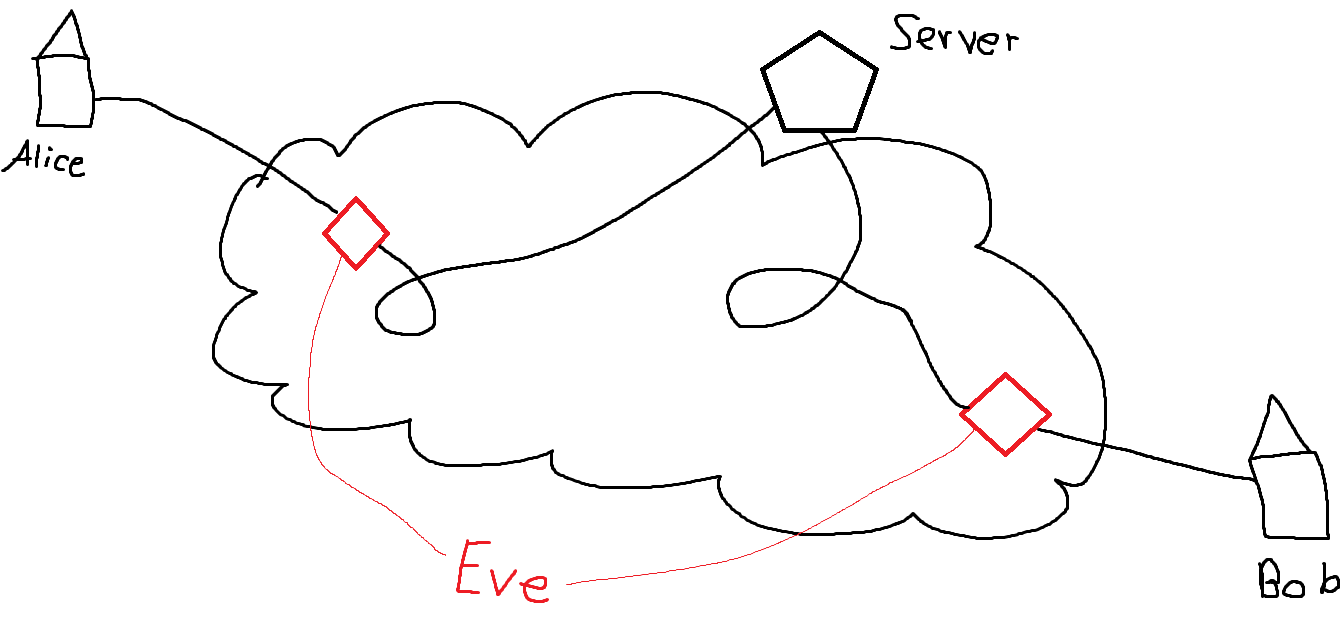
\includegraphics[scale=0.3]{Szenario.png}
        \pause

        \begin{itemize}
            \item
                Eve betreibt zwei Netzwerkknoten.
                \pause

            \item
                Sie beobachtet erst ein Paket von Alice zum Server und ein paar Millisekunden später eines vom Server zu Bob.
                \pause
                \begin{itemize}
                    \item[$\Rightarrow$]
                        Bei häufiger Kommunikation kann Eve mit Sicherheit wissen, dass die beiden miteinander schreiben.
                \end{itemize}
        \end{itemize}
    \end{frame}

    \begin{frame}
        \frametitle{Das Hydra-System (1)}
        \pause

        \begin{itemize}
            \item
                Nutzung von mindestens drei sogenannter \glqq Mixes\grqq, die onion-verschlüsselte Nachricht
                zwischen Client und Server (hier \glqq Rendezvous Node\grqq) vermitteln
                \pause

            \item
                Bestimmung des Pfades (\glqq Circuit\grqq) durch Client
                \pause
        \end{itemize}

        \centering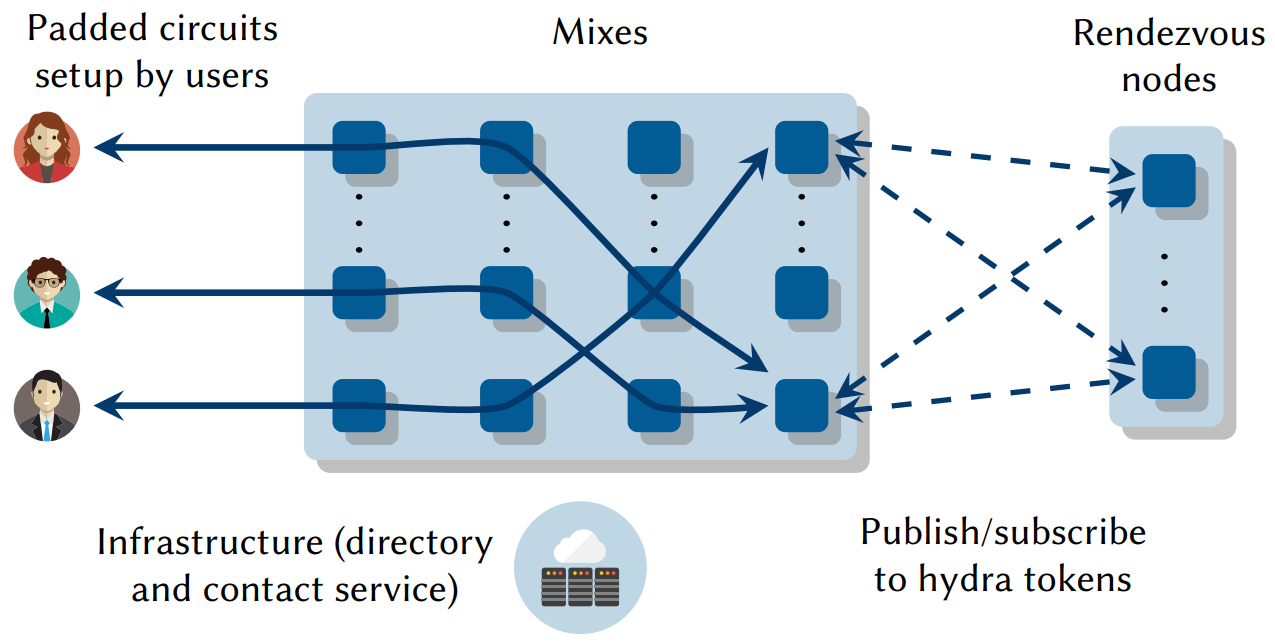
\includegraphics[scale=0.25]{hydra_design.png}
        \pause

        \begin{itemize}
            \item
                Zeit-synchronisiertes Senden aller Clients und Weiterleitung aller Mixes
        \end{itemize}
    \end{frame}

    \begin{frame}
        \frametitle{Das Hydra-System (2)}

        \centering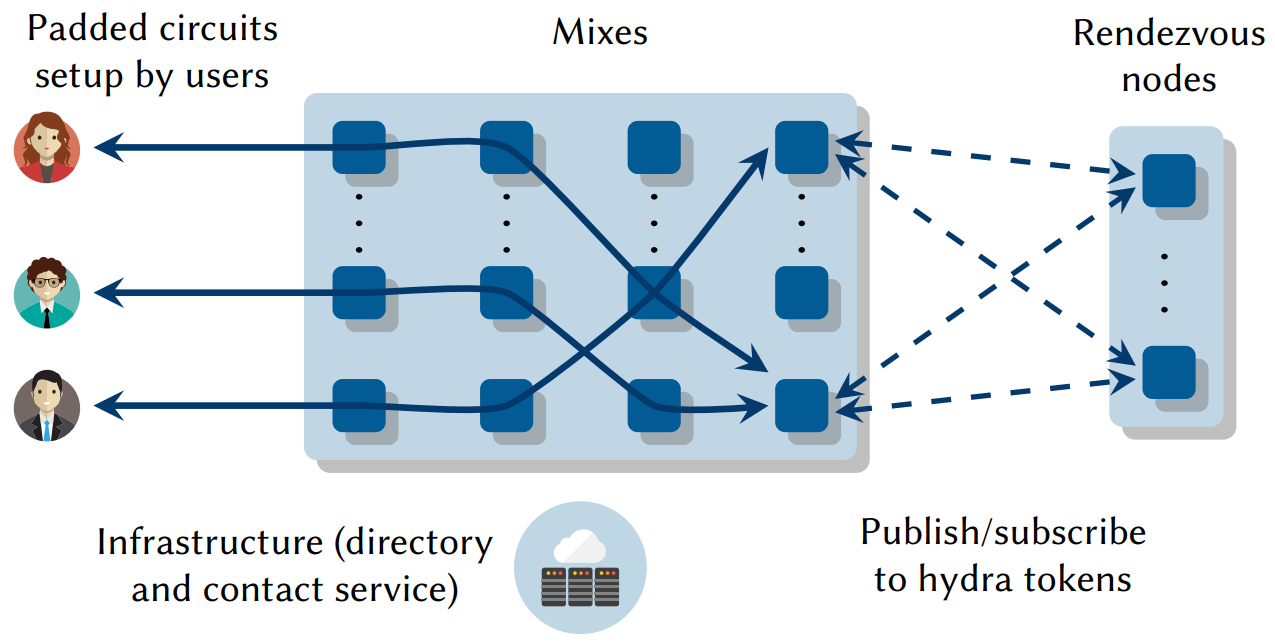
\includegraphics[scale=0.25]{hydra_design.png}

        \begin{itemize}
            \item
                Zeit-synchronisiertes Senden aller Clients und Weiterleitung aller Mixes
                \pause

            \item
                Senden von Dummy-Paketen mit zufälligem Inhalt, falls keine zu sendende Nachricht vorhanden
                \pause

            \item
                Fixe Paketgröße
                \pause
            \item[$\Rightarrow$]
                Timing-Angriffe wie auf voriger Folie nicht mehr möglich
        \end{itemize}
    \end{frame}

    \begin{frame}
        \frametitle{Das Hydra-System (3)}
        \pause

        Das Ziel ist die Gewährleistung von
        \begin{itemize}
            \item
                Beziehungsanonymität, d.h. die Geheimhaltung davon, wer wie oft mit wem schreibt, und
                \pause

            \item
                Ortsanonymität, d.h. die Geheimhaltung davon, welcher Nutzer zu welcher IP-Adresse gehört
                \pause
        \end{itemize}

        gegenüber jemandem, der
        \begin{itemize}
            \item
                im gesamten Internet Pakete beobachten, manipulieren, verzögern, wiederholen/kopieren und fälschen kann
                \pause

            \item
                mit einem Teil der User kooperiert und
                \pause

            \item
                einen (geringen) Teil der Mixe betreibt.
        \end{itemize}
    \end{frame}

    \begin{frame}
   		\frametitle{Unser Projekt - Der Hydra Client}
        \pause

   		Unser Projekt ist die Implementierung des Hydra Clients für Android.

   		Dieser muss
   		\begin{itemize}
   			\item Nachrichten gemäß des Hydra Protokolls senden und empfangen
   			\pause
   			\begin{itemize}
   				\item d.h. Nachrichten Ende-zu-Ende-verschlüsseln,
   				\pause
   				\item Nachrichten onion-verschlüsseln,
   				\pause
   				\item Setuppakete versenden und Circuts aufbauen,
   				\pause
   				\item  gewährleisten, dass alle Nachrichten ankommen und
   				\pause
   				\item  Dummypakete versenden können,
   				\pause
   				
   	 
   			\end{itemize}
   			\item sämtliche lokalen Daten geschützt speichern,
   			\pause
   			\item eine benutzerfreundliche GUI bieten und
   			\pause
   			\item auch im Hintergrund bei geschlossener App laufen.
   		\end{itemize}
   	\end{frame}
   	\begin{frame}
   		\frametitle{Abgrenzung}
   		\pause
        \centering{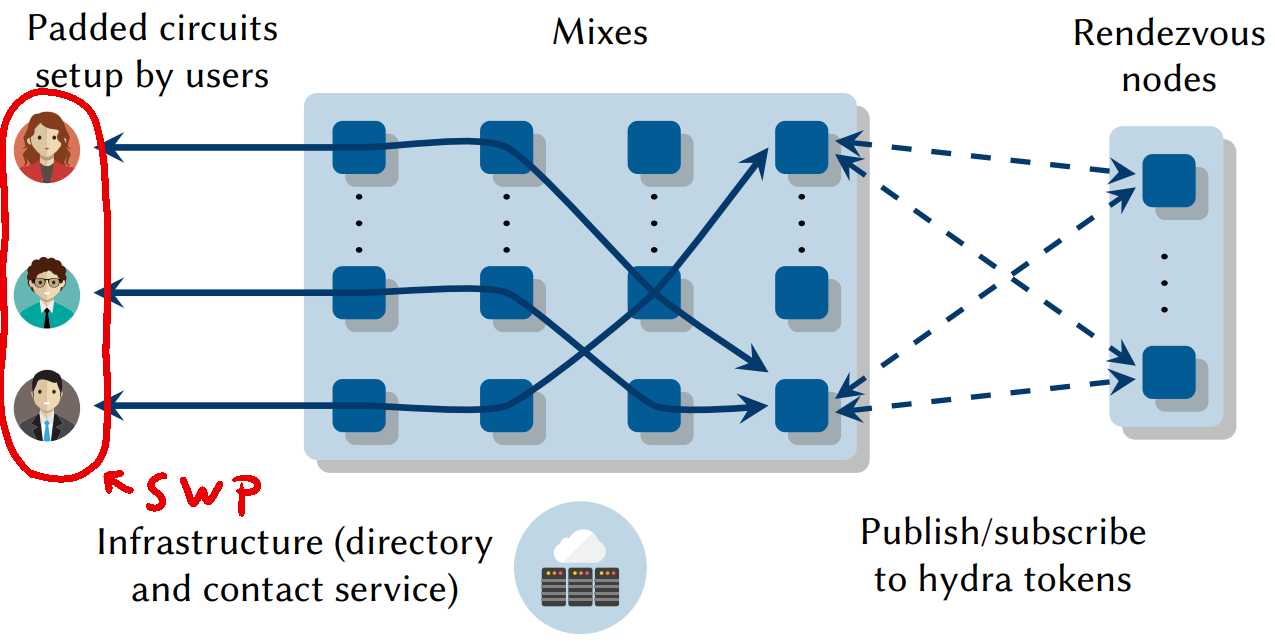
\includegraphics[scale=0.35]{hydra_design_modified_1.png}}
   		
        \raggedright
   		Unser Projekt beinhaltet explizit nicht irgendeine andere Komponente des Hydra Systems.
   	\end{frame}	
   
   \begin{frame}
   		\frametitle{Hinzufügen neuer Kontakte}
        \pause
   		\begin{itemize}
            \item
                Implementierung von Contact Discovery über das Hydra-System vorerst nicht geplant (Wunschfunktion)
                \pause

   			\item
                Austausch von Kontaktinformationen bei persönlichem Treffen über QR-Code
   		\end{itemize}
   \end{frame}

   \begin{frame}
   		\frametitle{Weitere wichtige Wunschfunktionen}
        \pause
   		\begin{itemize}
            \item
                Komprimierung von Nachrichten
                \pause
   			\item Fragmentierung von langen Nachrichten
                $\Rightarrow$ maximale Nachrichtenlänge größer als 240 Zeichen
   			\pause
   			\item Benachrichtigungen beim Empfangen neuer Nachrichten
                \pause
            \item
                Löschen einzelner Nachrichten aus dem Chatverlauf
   		\end{itemize}
    \end{frame}

    \begin{frame}
		\frametitle{Überblick interne Krypto Details}
        \pause
		
		\framesubtitle{Teil 1 - Schutz persistenter Daten}
		Mittels
		\begin{itemize}
			\item Android-interne Funktionen e.g. Android Key Storage
			\pause
			\item AES-Verschlüsselung von Daten mittels im Key-Storage
			gelagerter Schlüssel
		\end{itemize}
	\end{frame}

	\begin{frame}
		\frametitle{Überblick interne Krypto Details}
		
		\framesubtitle{Teil 2 - Schutz von Nachrichten}
		E2EE
		\pause $\Rightarrow$ AES Galois Counter Mode

		\centering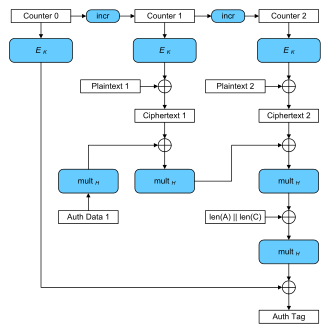
\includegraphics[scale=0.4]{AESGCM.png}
	\end{frame}

	\begin{frame}
		\frametitle{Überblick interne Krypto Details}
	
		\framesubtitle{Teil 2 -Schutz von Nachrichten}
		Onion-Verschlüsselung
	\pause $\Rightarrow$ Threefish x1024 in 12 Runden Feistel Netzwerk
	\centering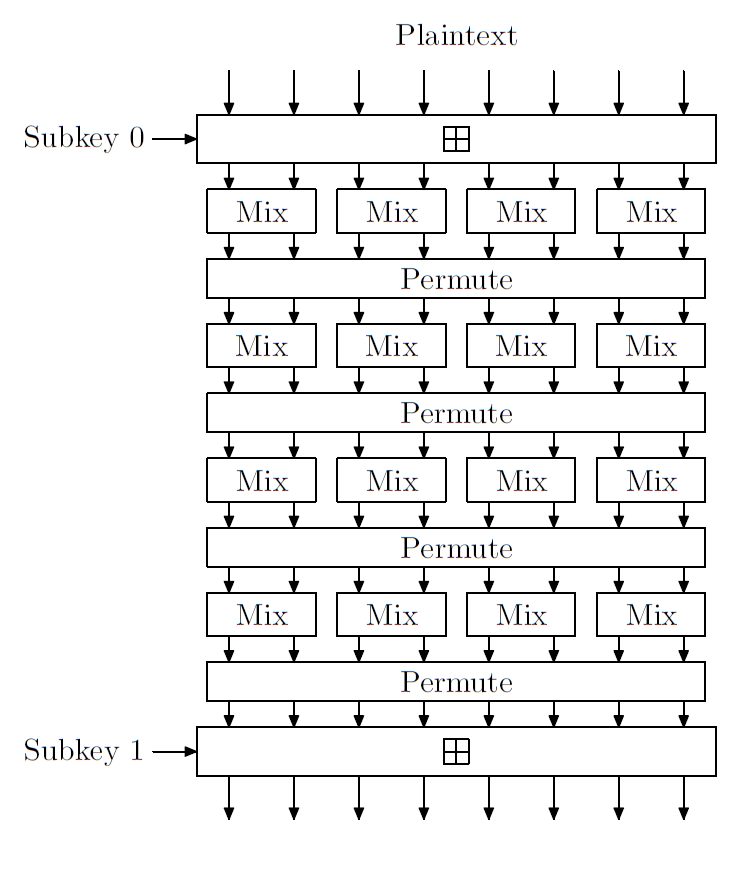
\includegraphics[scale=0.25]{Threefish.png}
	\centering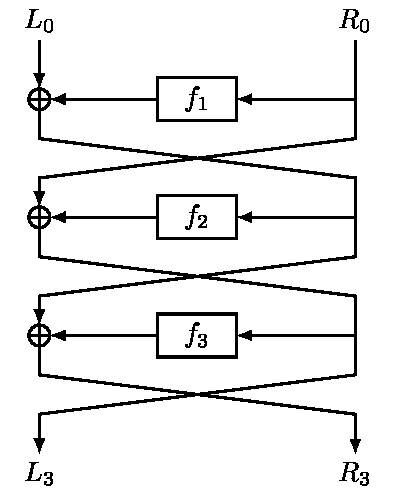
\includegraphics[scale=0.3]{Feistel_Network.png}
	
	\end{frame}
	
   		
   	

    \begin{frame}
        \frametitle{Verwendete Programmiersprachen}
        \pause

        \begin{itemize}
            \item
                Kotlin
                \begin{itemize}
                    \item
                        Kotlin und Java Standard für Android-Entwicklung

                    \item
                        Einfache Einbindung von Android-Features

                    \item
                        Nicht Java
                        \pause
                \end{itemize}

            \item
                C++
                \begin{itemize}
                    \item
                        Einfache Implementierung von Kryptographie und Netzwerkdingen

                    \item
                        Große Auswahl an vorhandenen Bibliotheken

                    \item
                        Erhöhte Portierbarkeit zu anderen Betriebssystemen, vor allem iOS
                \end{itemize}
        \end{itemize}
    \end{frame}

    \begin{frame}
        \frametitle{Ergebnis des Grobentwurfs: Lebenszyklus einer Nachricht}
        \pause

        \centering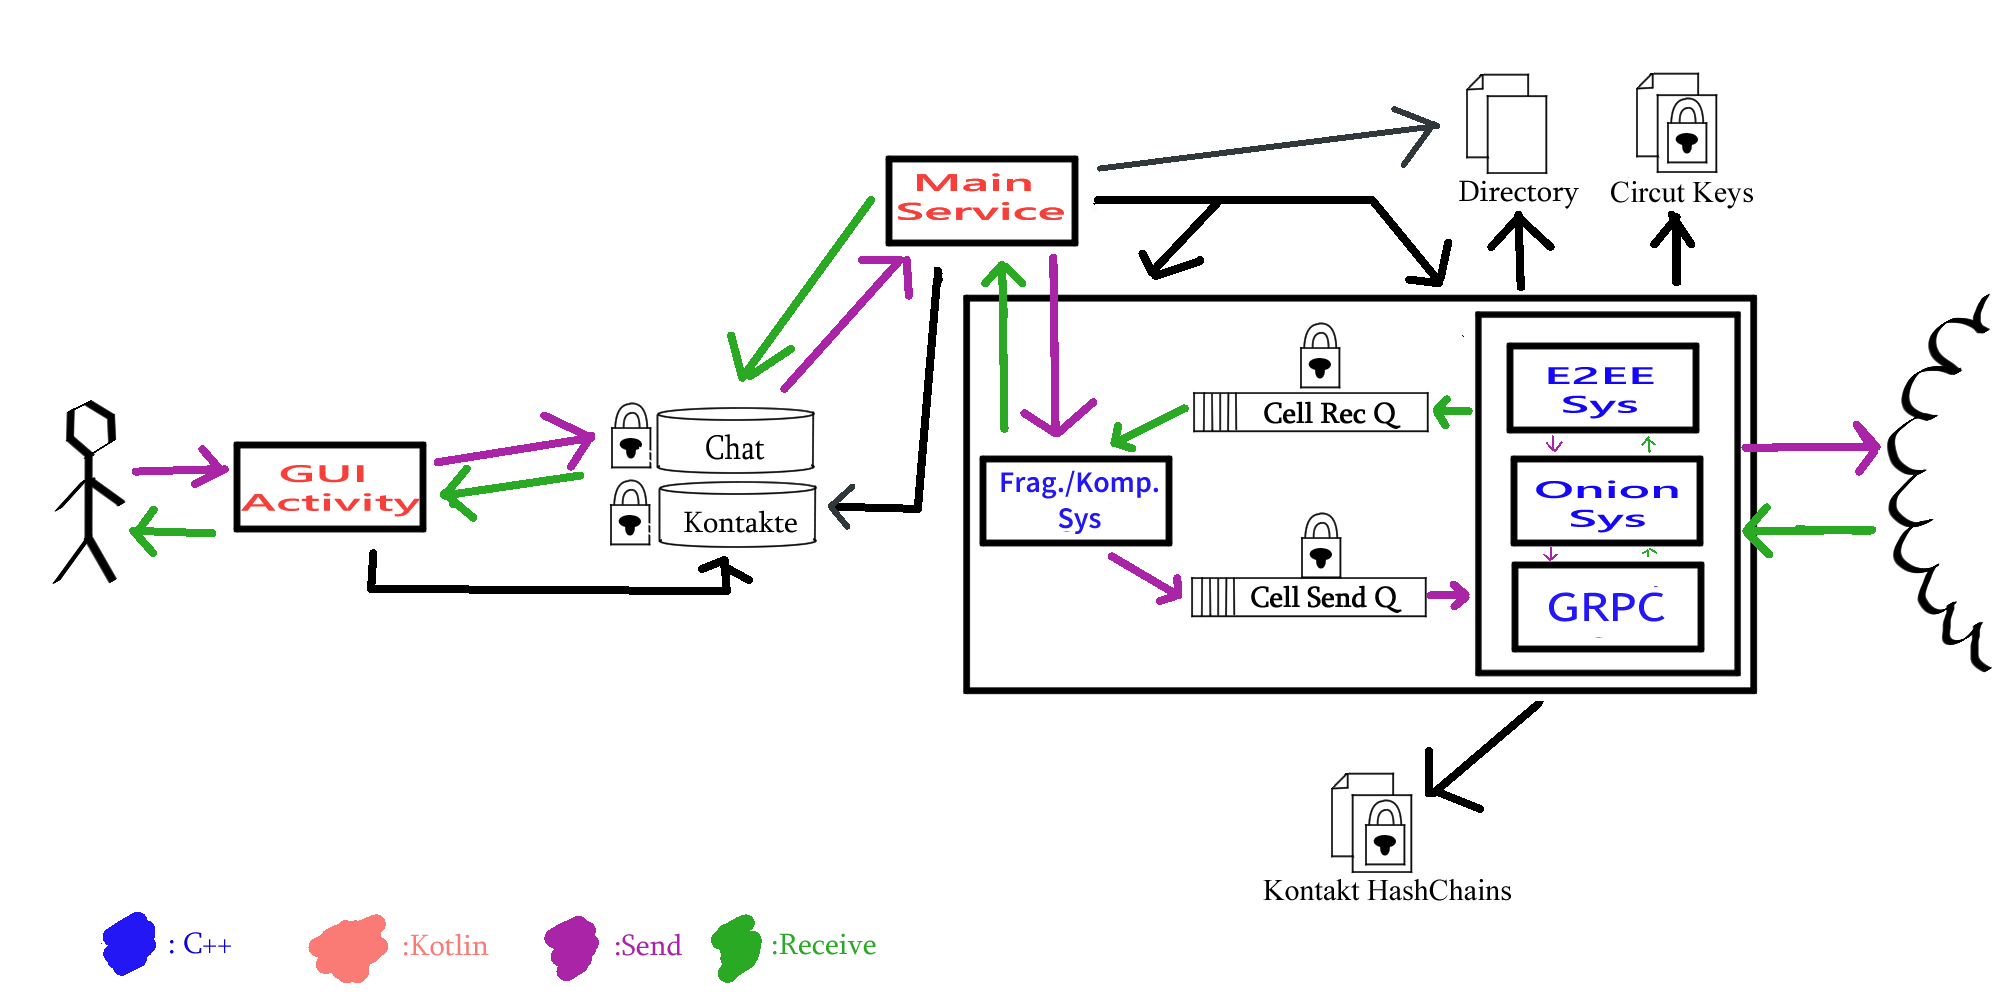
\includegraphics[scale=0.17]{Hydra_Cell_Cyclus.png}
    \end{frame}

	
	
	
	\begin{frame}
		\frametitle{Development Teams}
        \pause
			\begin{itemize}
			
					\item GUI Dev Team						
						\begin{itemize}
						
							\item Jonathan Skopp
							\item Jan Lemmen
							\pause
						\end{itemize}
					
					\item Datenbank Dev Team
						\begin{itemize}
						
							\item Alexander Wand
							\item Liam Pfannkuch
							\pause
							
						\end{itemize}
					
					\item Kryptogrphisches Dev Team
						\begin{itemize}
						
							\item Felix Kettnaker
							\item Carl-Christian von Dalnok
						\end{itemize}
				
			\end{itemize}

	\end{frame}



    % Kapitel Zeitplan
    \begin{frame}
        \frametitle{Zeitplanung/Meilensteine}
        \pause

        \begin{itemize}
            \item Bis 28.05.2020:
                Einfacher Prototyp mit provisorischer GUI, der Nachrichten unverschlüsselt senden und empfangen kann
                \pause
            
            \item Bis 10.06.2020:
                Alle Pflichtfunktionen fertig implementiert
                \pause
            
            \item Bis 18.06.2020:
                Bereits bekannte Fehler beheben, intensiv testen
                \pause

            \item Bis 02.07.2020:
                Betatest durchführen, mehr Fehler beheben
        \end{itemize}
    \end{frame}

	\begin{frame}
		\frametitle{Vielen Dank für Ihre Aufmerksamkeit}
		\framesubtitle{Noch Fragen?}
	\end{frame}

\end{document}
